\chapter{Containerization with Docker}
\label{cha:containerization-docker}
Docker is a tool for creating, provisioning and interacting with Linux Containers (LXC). LXC are a lightweight version of virtualization, which doesn't have the resource impact of a full virtualization, such as Operating System (OS) virtualization. The differences of LXC and a Virtual Machine (VM) are discussed in Section \vref{sec:docker-virtualization-vs-containerization}. Docker has become very popular over the past years, due to the fact, that it made it possible to easily work with LXC. Docker relies strongly on the principles of IaC which have been discussed in Chapter \vref{cha:iac}. When using Docker, Linux Containers are often referred to as Docker Containers\cite{Docker2018,LXC2018}. \\

Containerization is a key factor when hosting applications in the cloud, because the applications are normally packaged in images and run as containers on the cloud platform. Containerization provides features for a fast, effortless and consistent way of running applications in the cloud, which is discussed in the following section.

\section{The need for Containerization}
\label{sec:docker-need-for-containerization}
Containerization is a key factor for cloud platforms such as PaaS, where each application runs in its own isolated container. A container is an instance of an image, which represents the initial state of an application. A VM represents a full blown OS, whereby the OS provides a kernel, which is emulated by the Hypervisor on the host OS. A Hypervisor is a software, which can create, run, and manage VMs. A container uses the kernel provided by the host OS, and therefore there is no need for a kernel emulation. A container doesn't represent a full blown OS, but still provides features, normally provided by an OS, such a networking and storage\cite{DockerVirtScheepers2014}. \\ 

Containers are faster to create, to deploy, and easier to manage compared to VMs. Nevertheless, cloud platforms use virtualization for managing their infrastructure, whereby the containers run on the provisioned VMs. The usage of containers compared to the usage of VMs can reduce costs for hosting applications. Applications running in containers have less resource impact compared to applications running in VMs, because there is no virtualized OS and no need for kernel emulation. The creation, deployment and startup of containers are faster, because only the isolated process needs to be started and not a full blown OS. Docker is well supported by Integrated Development Environments (IDEs), which provide support for creating Docker Image-Definitions (Dockerfiles) and provisioning of Docker Containers on a local or remote host\cite{DockerFile2018}. \\

When enterprises have applied IaC to their systems, then the next logical step is to apply IaC to their applications as well. Applications running in containers profit from the IaC principles immutability, reproducibility, repeatability, and consistency, which have been discussed in Section \vref{sec:iac-principles}. Docker can be seen as an IaC tool, whereby the Dockerfiles represent the IaC templates and the Docker CLI represents the IaC tool. \\

When using Docker, developers define the process environment for their applications via a Dockerfile, and system administrators provide a VM with the Docker Engine, which is a shift of responsibility. Thus, system administrators have no control about the application environment anymore, which is not considered to be a problem, because the application processes are isolated from other processes, and cannot interfere them. Nevertheless, developers can profit from the deep Linux knowledge of system administrators, to define the Docker Images efficiently, to keep them small and secure. \\

The following sections will give an overview of the Docker technology, its architecture and artifacts.  

\section{Docker}
\label{sec:docker}
Docker is an open source software, which instruments kernel features like LXC. It provides a community edition for free, as well as an enterprise support for production use. The core part of the Docker technology is the Docker Engine, which is discussed in Section \vref{sec:docker-engine}. The Docker Engine is the part of the Docker technology that actually runs the containers. The Docker Images are managed in a so called Docker Registry, which is a repository for Docker Images. The most popular Docker Registry is Docker Hub, which is a free service, where anyone can publish Docker Images\cite{DockerRegistry2018}.

\subsection{Docker Engine}
\label{sec:docker-engine}
Figure \vref{fig:docker-engine} illustrates the Docker Engine architecture hosted on a Linux OS. The Docker Engine is build by layers, whereby each layer communicates with the layer beneath. The Docker Engine was initially designed for LXC exclusively, but has been ported to Windows as well. Docker Images and Docker Containers, which were created for a Windows OS, are not supported on a Linux OS and visa versa, because they use a different OS kernel. The Docker Images and Containers for a Windows OS differ from those for a Linux OS, but the principles of Docker Images and Docker Containers are the same.
\newpage

\begin{figure}[htbp]
	\centering
	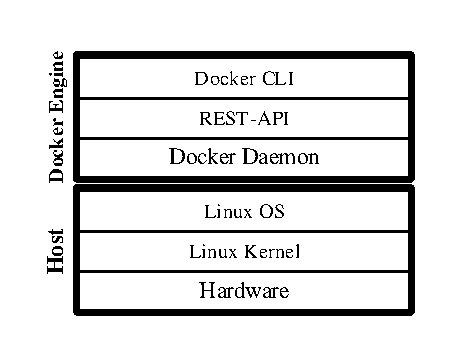
\includegraphics[scale=1]{images/docker-engine.pdf}
	\caption{Docker Engine architecture}
	\label{fig:docker-engine}
\end{figure} 

\mysubsubsection{Docker Daemon}
\label{sec:docker-daemon}
The Docker Daemon represents the background process, which creates, runs and manages the Docker Containers on the Docker Host, and is similar to a VM Hypervisor, but only on process level. The Docker Daemon strongly depends on the kernel of the host OS, therefore incompatibilities could cause the Docker Daemon to fail functioning. The communication with the Docker Daemon is performed via the Docker Engine exposed REST API,  because the Docker Engine is designed as a client server architecture. \\

\mysubsubsection{REST API}
\label{sec:docker-rest-api}
The REST API can be exposed via a Unix socket or a network interface, depending on the configuration of the Docker Daemon. If the REST API is exposed via a network interface, then it is recommended to secure the connection with client certificate authentication. If the Docker Engine and the Docker Client are located on the same host, then commonly the REST API is exposed via a Unix socket and doesn't need any special security. All commands executed via the Docker CLI are actually sent to the Docker Engine via its exposed REST API. \\

\mysubsubsection{Docker Command Line interface}
\label{sec:docker-cli}
The Docker Engine provides a Docker Command-Line-Interface (Docker CLI) for interacting with the Docker Daemon via a Linux shell. The Docker CLI itself is nothing more than a wrapper for the REST API, and communicates with the Docker Daemon via the exposed REST API. This is the most common way to interact with a Docker Daemon. The Docker CLI provides commands for creating container resources such as volumes and networks, managing Docker Images and Containers, and for provisioning the Docker Containers on the Docker Host. \\

\mysubsubsection{Docker Images}
\label{sec:docker-images}
Docker Images are defined via Dockerfiles, which contain instructions how to build the Docker Image. A Docker Image consists of immutable read-only layers, whereby one layer is created for each instruction in the Dockerfile. A layer can contain meta data or a file system state. Docker Images are hierarchical and inherit from another Docker Image, which is then called a base image. Docker Images support only single inheritance and the base image is defined via the \mentionedtext{FROM} instruction, which is the first instruction in the Dockerfile. Docker Images can be identified via their tags, whereby a Docker Image-Tag has the form of \mentionedtext{[url]<namespace>/<name>:<version>} e.g. \mentionedtext{docker.io/library/openjdk:8-alpine}. \\

\mysubsubsection{Docker Containers}
\label{sec:docker-containers}
A Docker Container is an instance of a Docker Image, whereby a new writable layer is appended, which contains all new or modified files. Deleting a Docker Container means, deleting the appended writable layer. Two Docker Containers, created from the same Docker Image, have their own appended writable layer, therefore the Docker Containers are isolated from each other. A Docker Container keeps running as long as the contained foreground process is running. Without a foreground process, the Docker Container stops immediately after the command was executed. The process running in the Docker Container is completely isolated from other processes, and is only allowed to use its assigned resources. \\

\mysubsubsection{Docker Volumes}
\label{sec:docker-volumes}
There are two ways to keep data persistent in Docker Containers. The first one is, to mount a host file system into the Docker Container, whereby the Docker Container depends on the specific host file system. The second one is, to use a Docker Volume, which abstracts the underlying storage type from the Docker Container, and is backed by a storage driver. Cloud storage providers can implement a driver, so that the data, stored in a Docker Volume, is actually kept persistent on a cloud storage. Another advantage of Docker Volume is, that the Docker Volumes can be moved between OS, which support Docker, and allow more detailed configuration.  

\mysubsubsection{Docker Network}
\label{sec:docker-network}
Docker provides networking features, whereby Docker Containers can be connected to each other via a Docker Network. Docker Networks are an abstraction of the actual networks, and are backed by a network driver, which implements the actual network type. The Docker Containers are not aware of the actual network type, the same as they are not aware of the actual storage type with Docker Volumes.

\subsection{Docker Architecture}
\label{sec:docker-architecture}
Figure \vref{fig:docker-architecture} illustrates the Docker architecture, which is a client server architecture. The design as a client server architecture is the reason why the communication to the Docker Daemon is performed via the exposed REST API. The Docker Client communicates with the Docker Daemon via the Docker CLI, whereby the Docker Client can be located on a remote host or on the Docker Host. The Docker Host runs the Docker Engine, which exposes the REST API, the Docker Client connects to. The Docker Engine manages the Docker Images and Docker Containers located on the Docker Host. The Docker Engine can push/pull Docker Images to/from a local/remote Docker Registry.

\begin{figure}[htbp]
	\centering
	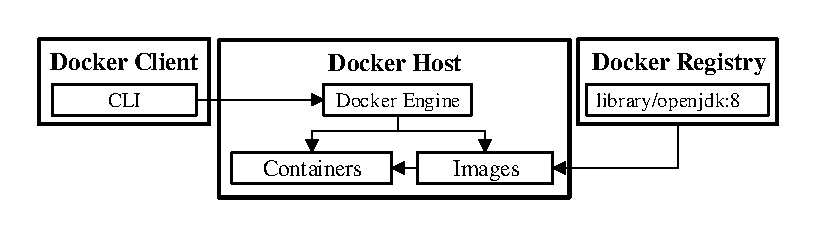
\includegraphics[scale=1]{images/docker-architecture.pdf}
	\caption{Docker architecture}
	\label{fig:docker-architecture}
\end{figure} 

\subsection{Docker Machine}
\label{sec:docker-machine}
The Docker Machine is a tool for managing local or remote Docker Hosts. With Docker Machine, an administrator can manage multiple Docker Hosts via a management server, without the need to connect to the Docker Host via a secure shell (SSH). The Docker Machine CLI provides all necessary commands for managing Docker Hosts. The Docker Engine provisions Docker Containers on a Docker Host and the Docker Machine provisions Docker Hosts on remote Linux hosts. With Docker Machine, a network of Docker Hosts can be managed, which is used by cloud platforms such as Openshift, to manage Docker Engines on the nodes within the Openshift Cluster\cite{DockerMachine2018}.  

\section{Virtualization vs. Containerization}
\label{sec:docker-virtualization-vs-containerization}
Before LXC the industry made use of OS virtualization to isolate their applications. A VM is managed by a Hypervisor, which is a software, which can create, run and manage VMs. The VM provides resources such as network and storage for the application, which is managed by the virtualized OS. Nevertheless, a VM represents a full blown OS, which itself has a resource impact, which adds to the resource impact of the running application. LXC on the other hand is a kernel technology, which provides resources such as network and storage to the application as well, but these resources are managed by the host OS, where the applications are running on.

\subsection{Virtual Machines}
\label{sec:docker-virtual-machines}
A VM is an instance of a Virtual Machine Image (VMI), which is managed by a Virtual Machine Monitor (VMM), which is also referred to as the Hypervisor. The actual difference between a VMM and a Hypervisor is where the software is installed on. If the software is directly installed on the Hardware, then the software is called a Hypervisor, if its installed on the Host OS then its called a VMM. The VM abstracts  an Guest OS from the Host OS, in particular from the underlying hardware. A VM contained Guest OS is not bound to the underlying hardware, because the Hypervisor performs a kernel emulation, which allows to virtualize any Guest OS on any hardware, if the Hypervisor supports it. The following Figure \vref{fig:docker-virtualization-architecture} illustrates the architecture of applications running on a virtualization infrastructure.

\begin{figure}[htbp]
	\centering
	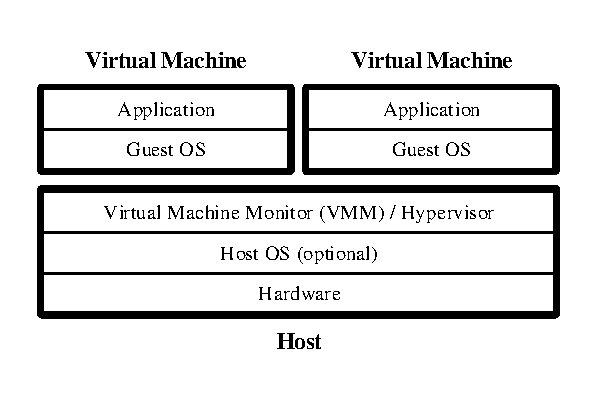
\includegraphics[scale=1]{images/docker-virtualization-architecture.pdf}
	\caption{Architecture of virtualized applications}
	\label{fig:docker-virtualization-architecture}
\end{figure} 

Glauber Costa's started the abstract of his talk at the LinuxCon 2012 with the humorous note \mentionedtext{"I once heard that Hypervisors are the living proof of operating system's incompetence"}. With this note he expressed, that OS weren't able to provide proper isolation for applications, and therefore the industry started to provide an OS instance for each application. This has been overcome with the upcoming of LXC, which provide the proper isolation of applications on the same OS, which made the need for an OS instance for each application obsolete\cite{LxConCosta2012}.

\subsection{Linux Container}
\label{sec:docker-linux-container}
The appearance of LXC has eliminated the shortcoming of the Linux OS, which wasn't able to isolate applications properly, which lead to OS virtualization for application isolation. LXC provide the feature of isolating applications running on the same OS, without the need of a kernel and hardware emulation as it is done with OS virtualization. As illustrated in Figure \vref{fig:docker-container-architecture}, the application process, binaries, and libraries are bundled into the container, and are isolated from other containers. Each container gets a portion of the global resources such as CPU cycles and memory assigned, and cannot consume more as it has been assigned to. Without LXC it is possible that one process takes over all available system resources, whereby other processes would starve.

\begin{figure}[htbp]
	\centering
	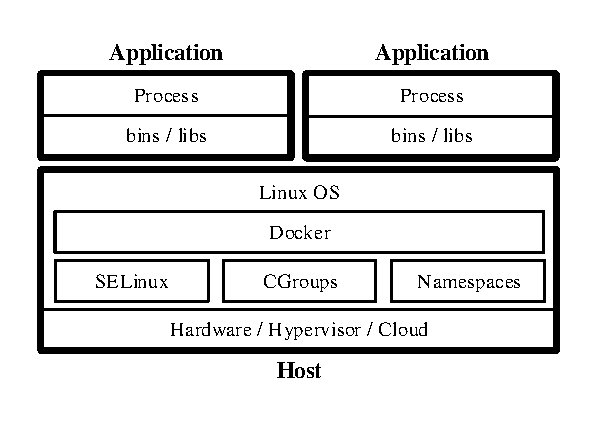
\includegraphics[scale=1]{images/docker-containerized-architecture.pdf}
	\caption{Architecture of containerized applications}
	\label{fig:docker-container-architecture}
\end{figure} 

The following sections will discuss the two most important kernel features for LXC, Cgroups and Namespaces, which provide resource control and isolation. 

\mysubsubsection{Cgroups}
Cgroups stands for control groups, and Cgroups provide the ability to aggregate processes, their child processes and threads, to groups, which are managed in a tree structure. Each group gets a portion of the global resources such as CPU cycles or memory assigned, whereby it is guaranteed, that a group and its managed processes cannot consume more resources as the group has been assigned to. Each process running in a container is assigned to a group, whereby a process cannot steal resources from another process anymore, because the resource assignments of a group, managed by Cgroups, prevents this from happening\cite{KernelCGroupsV12018, KernelCGroupV22015, IntelLXCHyperVisor2014}. \\

\mysubsubsection{Namepsaces}
Cgroups manage how many resources can be used by processes in a group, and Namespaces manage the view of the system to processes. A container is managed in its own namespace, and therefore the container has a limited view of the system, such as networks and process ids (PIDs). Namespaces are a fundamental concept of LXC, and Namespaces provide the isolation between containers\cite{LinuxNamespaces2018, IntelLXCHyperVisor2014}. \\

The following chapter will discuss Kubernetes, which is an orchestrator for Docker Containers, and allows to manage Docker Containers in a clustered environment. 
 

